\section{Namespace Schemas}
\label{sec:namespace-schemas}

\begin{figure}[tb]
  \centering
  \begin{subfigure}[b]{1\linewidth}
    For \(n\) processes on \(m\) servers:
    \begin{itemize}
      \setlength\itemsep{-0.5em}
      \item[] \texttt{\# of dirs =} \(m \times \texttt{mkdir()}\)
      \item[] \texttt{\# of file =} \(2 \times n \times m\)
      \item[] \texttt{\# of file per dir =} \(n/m\)
    \end{itemize}
    \caption{Function schema for PLFS\vspace{1em}} \label{fig:plfs}
  \end{subfigure}

  \begin{subfigure}[b]{1\linewidth}
      \footnotesize
      \begin{minted}[xleftmargin=1em]{lua}
local box require 'box2d'
for i=_x,_x+x do     -- iterate over the
  for j=_y,_y+y do   -- given bounding
    for k=_z,_z+z do -- box coordinates
      if temperature>30 then
        -- partition object list one way, e.g.,
        b0, b1 = box.nsplit(2)
      else
        -- partition a different way, e.g.,
        b0, b1, b2, b3 = box.nsplit(4)
      end
end end end
return obj_list
     \end{minted}
      \caption{Code schema for SIRIUS\vspace{1em}} \label{fig:sirius}
  \end{subfigure}

  \begin{subfigure}[b]{1\linewidth}

\noindent\texttt{pointer\_schema}: \texttt{(o0, o2, o9)}

\noindent\texttt{code\_schema}:

      \centering
      \footnotesize
      \begin{minted}[xleftmargin=1em]{c++}
void recurseBranch(TObjArray *o) {
  TIter i(o); 
  for(TBranch *b=i.Next(); i.Next()!=0; b=i.Next()) {
    processBranch(b);
    recurseBranch(b->GetListOfBranches());
  }
}
      \end{minted}
      \caption{Pointer and Code schemas for HEP\vspace{1em}} \label{fig:hep}
  \end{subfigure}
\caption{Namespace schemas that generate subtrees for 3 motivating examples.\label{fig:use-cases}}
\end{figure}

%local box require 'box2d'
%o = {}; i = 1   -- o: object list
%for _x=x,x+size do for _y=y,y+size do 
%  if temperature>30 then
%    box0=box.nsplit(0,2,h,x,y,z,size)
%    box1=box.nsplit(1,2,h,x,y,z,size)
%    o[i]=box0(); i=i+1
%    o[i]=box1(); i=i+1
%  else o[i] = _x.._y..z.."_0"; i=i+1 end
%end end
%return o
 

%char *tn = getTreeName().c_str();
%TTree* t = (TTree*) root->Get(tn);
%TIter i(t->GetListOfBranches());
%for(TBranch *b = i.next();
%    i.Next() != 0;
%    b = (TBranch*) i.Next())
%  recurseBranch(b->GetListOfBranches());

For three domain-specific applications and use-cases, we have identified
different scalability challenges:

\begin{enumerate}
  \item namespaces with many requests
  \item namespaces managed by remote servers
  \item namespaces that are too large
\end{enumerate}

Tintensfisch addresses all three challenges by having clients/servers store
namespace schemas, which generate file system metadata. This approach reduces
RPC load (addresses challenges 1 and 2) and facilitates lazy file system
metadata generation when the metadata is needed (addresses challenge 3).
Tintenfisch relies on the user to design effective namespace schemas that
leverage domain-specific knowledge to get the highest performance. This
programmable storage approach~\cite{sevilla:eurosys18-malacology} helps
application developers tailor the storage system to the use case without having
to design a new storage system from scratch.

Tintenfisch is built on Cudele~\cite{sevilla:ipdps18-cudele} so a
centralized, globally consistent metadata service (either a single metadata
server or a cluster of active-active metadata servers) provides clients with
the root inode of the subtree of interest and clients can do metadata IO
locally with the consistency/durability semantics they require. In Tintenfisch, 
the namespace schema is stored in the directory inode of the root of the
subtree that the client cares about. We use the ``file type" interface from the
Malacology~\cite{sevilla:eurosys17-malacology} project to facilitate this
domain-specific functionality. This is similar to push-down predicates in
databases, where the application is providing domain-specific knowledge that
the storage system knows how to leverage.  We have defined three types of
namespace schemas: formula, code, and pointers.

\subsection{Formula Schema} 

For this schema, a formula that generates the file system namespace is stored
in the inode. This formula takes domain-specific information as input and
produces a list of files and directories.  For example, because PLFS clients
deterministically create files and directories based on the number of clients,
Tintenfisch can use a formula schema like the one in Figure~\ref{fig:plfs}. The
function takes as input the number of processes and hosts in the cluster and
outputs the number of directories, the number of files, and the number of files
per directory.  For the example, the namespace drawn in
Figure~\ref{fig:tree_plfs} can be generated with the formula in
Figure~\ref{fig:plfs} using an input of 3 hosts each with 1 process. The output
is 3 directories and 6 files, with 2 files per directory.  With this namespace
schema, clients can open just the container inode and then compute and access
its contents without \texttt{lookup()} and \texttt{open()} RPCs to a
centralized metadata service.

%For \(n\) processes on \(m\) servers:
%\begin{itemize}
%  \item[] \texttt{\# of dirs =} \(m \times \texttt{mkdir()}\)
%  \item[] \texttt{\# of file =} \(2n \times \texttt{create()} [+ 2n \times \texttt{lookup()}]\)
%  \item[] \texttt{\# of file per dir =} \(n/m\)
%\end{itemize}

\subsection{Code Schema}

Sometimes the namespace schema logic is too complex to store as a single
function or requires external libraries to interpret metadata. For example, the
SIRIUS use case constructs the namespace using domain-specific partitioning
logic written in Lua (for sandboxing purposes).  Tintenfisch provides a code
schema that gives users the flexiblity to write programs that generate the
namespace.

A code schema for the SIRIUS project is shown in Figure~\ref{fig:sirius}.  A
namespace is constructed by iterating through the bounding box coordinates and
checking if a threshold temperature is eclipsed. If it is, then extra names
are generated using the \texttt{box2d} Lua package.  Although the partitioning
function itself is not realistic, it shows how code schemas can accomodate
domain-specific data layout policies that are complex and/or require external
libraries.  

\subsection{Pointer Schema} 

Sometimes there is no formal specification for the namespace. For example, the
ROOT framework uses self-describing files so headers and metadata need to be
read for each ROOT file. In these scenarios, a code schema is insufficient for
generating the file system namespace because all necessary metadata is in
objects scattered in the object store. Pointer schemas reference data in
scalable storage and avoids storing large amounts of metadata in inodes, which
is a frowned upon in distributed file systems like
CephFS~\cite{docs:cephinternals}.

For example, a code schema containing library code for the ROOT framework
\emph{and} a pointer schema for referencing the input to the code can be used
to describe a ROOT file system namespace. The pointer schema would point to
objects in the object store that contain the necessary metadata for
constructing the file system namespace. This is shown in Figure~\ref{fig:hep};
clients requesting Branches would follow the pointer schema to the objects
containing metadata and would read them to locate Baskets using the code
schema. An added benefit to this solution is that Tintenfisch can lazily
construct parts of the namespace as needed, which avoids the problem of running
out of inodes discussed in Section~\ref{sec:hep_namespace-description}.

\subsection*{A Fresh, Unorthodox, Unexpected, Controversial, and Counterintuitive Idea}

Global file systems can be scalable if programmed correctly. For example, the
following notions are out-dated:

\begin{itemize}
  \setlength\itemsep{-0.5em}

  \item robust so they are fast... but we show that today's apps are so large
  that we need to specialized storage systems

  \item general because they have been around for so long... but we show that
  most apps don't need fs metadata

  \item subject to data IO performance... but we show that metadata is slow

\end{itemize}


%In this section, we show how clients and metadata servers communicate using the
%Pattern PLFS language and present our
%storage system that adapts to the wokload
%(Section~\ref{sec:adapting-to-the-workload-with-cudele})).  Other destructive
%solutions include changing the storage system and altering the application.
%
%\subsection{Adapting to the Workload with Cudele}
%\label{sec:adapting-to-the-workload-with-cudele}
%
%\begin{figure}[tb]
%\centering
%  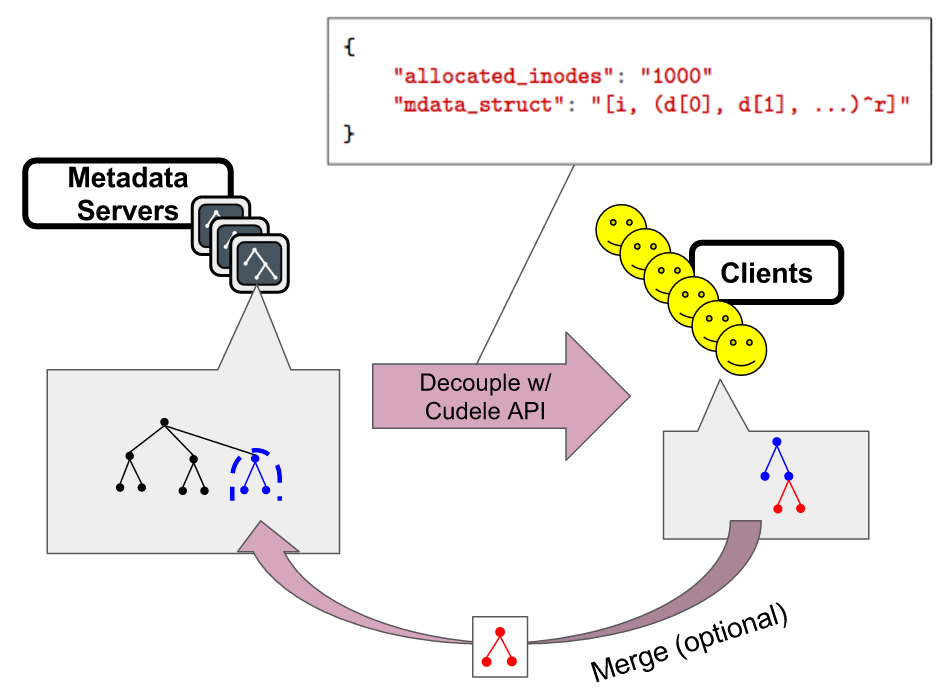
\includegraphics[width=90mm]{figures/arch.png} 
%  \caption{System XX lets clients optimize performance by telling the storage
%  system about the workload. Clients can specify a Structured Namespace (blue
%  subtrees and Section~\ref{sec:structured-namespaces}) or by merging file system
%  metadata from an Unstructured Namespace (red subtree and
%  Section~\ref{sec:unstructured-namespaces}).}\label{fig:arch}
%\end{figure}
%
%% What is Cudele
%Cudele is a file system with programmable consistency and durability. Clients
%use an API to decouple existing subtrees from the global namespace; metadata
%operations from the other clients targeted at the decoupled subtree can be
%programmed to be blocked or marked as overwritable. With the decoupled subtree
%in hand, the client can do metadata operations locally. Upon completion, the
%client can merge the subtree back into the global namespace. 
%
%% Why Cudele is a good fit for implied namespaces
%Cudele has the mechanisms for understanding the file system metadata language
%and adapting to the workload.  Figure~\ref{fig:arch} shows how clients decouple
%the namespace with the Cudele API, specifying how many extra inodes they want
%and the structure for the namespace they intend to create. The metadata server
%and client both know about the metadata in the blue subtree, requiring no RPCs,
%and if the client creates more metadata (red subtree), it can merge it back
%into the global namespace.  This model lets users enjoy the simplicity of
%global namespaces and the high performance of node-local operations.  We extend
%the API to support the declaration of structured namespaces and leverage the
%existing API to merge unstructured namespaces. 
%
%\subsubsection{Structured Namespaces}
%\label{sec:structured-namespaces}
%
%% What is a structured namespace
%A structured namespace is created according to a pattern. If both the client
%and metadata server knows the pattern, they can create the metadata
%independently. This has two benefits: (1) it reduces RPCs which improves
%performance and reduces network traffic and (2) it allows the client and server
%to operate in parallel.  The patterns that Cudele understands are shown in
%Listing~\ref{src:example} and the programmable interfaces are shown below.
%There are two parameters for unstructured namespaces: \texttt{pattern} and
%\texttt{trigger}. 
%
%\subsubsection{Trigger: Start Namespace Construction}
%
%% How does trigger work and why do we neet it
%\texttt{trigger} specifies when to start the namespace construction on the
%metadata server.  The metadata reconstruction can be asynchronous and saving
%this resource intense process for later can have better performance. To
%facilitate the exploration of different trigger policies, we make the value for
%the \texttt{trigger} parameter programmable.  Administrators inject Lua code
%that specifies or calculates thresholds for when to start namespace
%construction. Although we make this programmable, we do not make any
%conclusions about the best trigger time and leave the exploration of this space
%as future work.
%
%% example
%In Listing~\ref{src:example}, the trigger is:
%\begin{listing}
%\begin{minted}[frame=single,
%               framesep=2mm,
%               xleftmargin=10pt,
%               tabsize=2]{lua}
%{
%  if MDSs[whoami]["cpu"] > 30
%}
%\end{minted}
%\label{src:thresh}
%\end{listing}
%
%which means that construction of the namespace will start if current MDS
%(\texttt{whoami}) has a CPU utilization (\texttt{``cpu"}) above 30\%.
%
%% Drawbacks: consistency
%Triggering construction asynchronously can improve performance because the
%process can be deferred until the system has less load. However, this
%performance gain comes at the cost of consistency. Even if the construction is
%triggered immediately, the metadata is eventually consistent; other clients see
%outdated metadata because the namespace is sitting on the client. Delaying the
%trigger improves the liklihood that system finds a window of low load but also
%increases the latency of other clients.\\
%
%\noindent\textbf{Implementation}: we re-use the polling and embedded Lua
%virtual machine in Mantle~\cite{sevilla:sc15-mantle} to implement the trigger
%interface. By default, every 10 seconds the metadata server checks if the
%condition for triggering is satisfied by executing the Lua code. Mantle has
%variables exposed for administrators to explore load balancing policies; just
%like this work, some of these policies need to identify overloaded metadata
%servers so we re-use all those variables.  Some of the more useful variables
%include:
%
%\begin{itemize}
%  \item Memory Usage
%  \item CPU Utilization
%  \item Request Rate
%  \item Queue Depth
%  \item Server Tags: whoami, i
%\end{itemize}
%
%\subsubsection{Pattern: Express Namespace}
%\label{sec:pattern-express-namespace}
%
%% How does pattern work and why do we need it
%\texttt{pattern} describes the metadata layout of the Structured Namespaces. It
%is the same language used in~\cite{he:hpdc13-plfs-patterns}. When the metadata
%server starts a namespace construction, it creates all the file system metadata
%generated by this formula. As a refresher, the pattern in Listing~\ref{src:example}:
%
%  \[[i, (d[0], d[1], ...)^r]\]
%
%means that there are \(r\) entries in the PLFS index file, where the first
%entry has a physical offset of \(i\) and lengths of \(d\), where the pattern in
%\(d\) repeats. \\
%
%% WTF -- this doesn't give file system metadata! ARGGGGG is it file creations
%% or index files shit?
%
%% Drawbacks
%
%\noindent\textbf{Implementation}: Another big fat TODO.
%
%\begin{listing}
%\begin{minted}[frame=single,
%               framesep=2mm,
%               xleftmargin=10pt,
%               tabsize=2]{js}
%{
%  <!-- Structured Namespace Pattern !-->
%  "S_pattern": "[i, (d[0], d[1], ...)^r]",
%  
%  <!-- Structured Namespace Trigger !-->
%  "S_trigger": "if MDSs[whoami]["cpu"] > 30",
%  
%  <!-- Untructured Namespace Allocated Inos !-->
%  "US_alloci": "1000",
%}
%\end{minted}
%\caption{Using the Cudele API to express metadata structure, which is
%understood by both the server and client.}
%\label{src:example}
%\end{listing}
%
%\subsubsection{Unstructured Namespaces}
%\label{sec:unstructured-namespaces}
%
%\subsubsection{Migrating Metadata Construction}
%\label{sec:migrating-metadata-construction}
%
